\section{U002 Latency hiding and physical storage lifetime}
\label{sec:u002}

Latency hiding requires work to be outstanding before it is needed. It does not follow that every outstanding operation must occupy its eventual compute destination for the whole wait. The distinction is the subject of U002: when must a physical payload location be owned, what state must remain while it is not owned, and when is reuse safe? Compiler lifetime planning, software multibuffering, explicit dataflow queues, and hardware-managed logical-to-physical binding are different answers to this question. Their comparison requires separate accounting for requests, returned data, allocation pools, individual values, and genuinely live compute state.

This distinction is easy to lose in attention. A kernel can prefetch a future K block while retaining Q, running maxima and denominators, an output accumulator, and other K/V blocks being consumed. Some storage contains useful live data; some is reserved for a future arrival; some exists because the enclosing kernel allocated a fixed pool. Reclaiming one consumed K slot does not free the pool, and making part of a score tile readable does not establish that its physical storage can be released one cell at a time. The relevant objective is to reduce avoidable residency while retaining correct ownership and a completion path for every admitted operation.

\subsection{Five intervals describe one asynchronous load}

For a value $i$ with logical payload size $b_i$ and charged physical allocation size $s_i$, distinguish the following intervals. \emph{Request tracking} begins when the system must remember an operation's identity and ends when the associated tracking state is no longer required. \emph{Returned-data residence} covers a response that has arrived but has not yet been placed in or consumed from its next storage location. \emph{Pool allocation} is the interval during which a larger capacity reservation exists. \emph{Value ownership} is the interval during which a particular slot belongs to value $i$ and cannot be overwritten by another value. \emph{Compute-live residence} covers valid payload held in compute-local storage that is still required by remaining consumers. Returned data waiting elsewhere are also logically live; this last category isolates their residency after placement in compute storage. The intervals can overlap. The exact boundaries depend on the interface; these categories are an accounting framework rather than a universal implementation diagram.

Let $a_i$ be physical destination acquisition and $f_i$ safe release. For distinct, non-aliased allocations, let $s_i$ include the physical envelope, padding, and capacity rounding charged to the value. The destination occupancy attributable to values is
\begin{equation}
 D(t)=\sum_i s_i\,\mathbf{1}_{[a_i,f_i)}(t),
 \qquad
 A_D=\int D(t)\,dt=\sum_i s_i(f_i-a_i),
 \label{eq:u002-byte-time}
\end{equation}
where $A_D$ is a byte-time measure. It exposes long avoidable holding intervals, but it is not an area estimate. Physical implementation also depends on peak simultaneous demand, banking, ports, fragmentation, and whether different pools can share capacity. If a fixed pool has capacity $C$, slot reuse can reduce value occupancy within it while leaving the allocated capacity $C$ unchanged.

Similarly, request count $N_{\mathrm{req}}(t)$ is not payload capacity. A request record might hold an address, length, tag, generation, and status rather than a complete data tile. Return buffers can have their own allocation and backpressure rules. If the same physical memory backs several roles, their occupancy must be counted as a union of physical regions rather than summed twice. If they are disjoint, each region's capacity and lifetime belongs in the ledger. Neither ``bytes in flight'' nor ``number of buffers'' is sufficiently precise by itself.

\begin{figure}[tb]
\centering
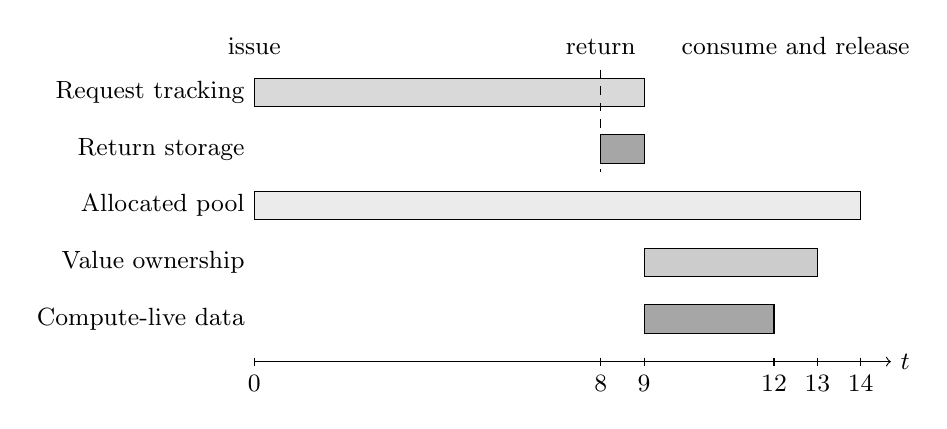
\begin{tikzpicture}[x=0.55cm,y=0.72cm,every node/.style={font=\small}]
 \node[anchor=east] at (0,4) {Request tracking};
 \node[anchor=east] at (0,3) {Return storage};
 \node[anchor=east] at (0,2) {Allocated pool};
 \node[anchor=east] at (0,1) {Value ownership};
 \node[anchor=east] at (0,0) {Compute-live data};
 \draw[fill=black!15] (0,3.75) rectangle (9,4.25);
 \draw[fill=black!35] (8,2.75) rectangle (9,3.25);
 \draw[fill=black!8] (0,1.75) rectangle (14,2.25);
 \draw[fill=black!20] (9,0.75) rectangle (13,1.25);
 \draw[fill=black!35] (9,-0.25) rectangle (12,0.25);
 \draw[->] (0,-0.75)--(14.7,-0.75) node[right] {$t$};
 \foreach \x in {0,8,9,12,13,14} {
  \draw (\x,-0.68)--(\x,-0.82);
  \node[below] at (\x,-0.83) {\x};
 }
 \node[above] at (0,4.5) {issue};
 \node[above] at (8,4.5) {return};
 \draw[dashed] (8,4.4)--(8,2.6);
 \node[above] at (12.5,4.5) {consume and release};
\end{tikzpicture}

\caption{An illustrative late-binding lifecycle. The response arrives at $t=8$, destination ownership begins at $t=9$, the last modeled computation consumes the data by $t=12$, and ownership is released at $t=13$. The enclosing pool remains allocated until $t=14$. These times are invented for explanation; tracking may last longer in other implementations.}
\label{fig:u002-lifetimes}
\end{figure}

For the example in Figure~\ref{fig:u002-lifetimes}, suppose the logical payload and charged allocation are both $16$ KiB. An early-bound destination held from $t=0$ through $t=13$ accounts for $208$ KiB-time units; a destination acquired at $t=9$ accounts for $64$. The difference, $144$ KiB-time units, is an illustrative reduction in that destination's reservation interval. It is not a claim of saved SRAM area or energy. The late-bound design also requires return storage during $[8,9)$, may temporarily hold two copies during movement, and needs mapping and arbitration state. If its enclosing pool is unchanged, physical capacity may be identical. If binding is delayed until $t=11$, the consumer may start later; the smaller destination interval can then accompany worse latency. A residency result must therefore be reported together with completion time and occupancy elsewhere.

\subsection{Outstanding work and live payload impose different bounds}

For a steady stream of fixed-size requests with average request rate $\lambda$ and average request latency $L$, the average outstanding count is $\lambda L$ under the usual stable-flow assumptions. At a delivered byte rate $B$, the associated bandwidth--latency product is $BL$. For variable request sizes, let $\ell$ be per-request latency, with $L=\mathbb{E}[\ell]$. Mean outstanding bytes are $\lambda\mathbb{E}[b\ell]=B L_b$, where $L_b=\mathbb{E}[b\ell]/\mathbb{E}[b]$ is byte-weighted mean latency. This is a statement about outstanding traffic, not proof that $BL$ bytes occupy a particular SRAM. Bytes may still reside at the source, be traversing a network, wait in return storage, or have arrived at their destination. The architecture determines which of these states requires an explicit payload reservation.

An idealized pipeline producing one tile every $I$ time units needs roughly $\lceil L/I\rceil$ requests in flight to cover a fixed latency $L$, before additional constraints are considered. Burstiness and variable service can require more slack or force stalls. A finite queue cannot guarantee a target throughput for arbitrary unbounded delay. Equally, adding destination buffers cannot overcome a sustained bandwidth deficit: if the consumer needs $b/I$ bytes per unit time and the supply can deliver only $B<b/I$, eventual starvation remains.

There is also an independent lower bound from truly live values. For a chosen algorithm and schedule without spilling or recomputation, all values needed by future consumers must remain available somewhere. If $\mathcal{L}(t)$ is the set of such values, then storage across the locations retaining them must accommodate their live payload, with aliases counted once. Late binding can remove an unnecessary pre-arrival destination hold; it cannot remove the information content of $\mathcal{L}(t)$. A different algorithm may reduce this set through streaming, recomputation, or changed accumulation, but its extra compute and traffic must then be charged to that algorithm.

This is why the running state in Equation~\ref{eq:u001-online-attention} matters. A K block can often be released after its last relevant QK use, while an output accumulator and row statistics remain necessary across subsequent KV blocks. Treating all of these as identically short-lived tiles exaggerates what an allocator can reclaim. The meaningful question is which values are held before they are present, after their final use, or in unnecessarily duplicated form, and whether shortening those intervals changes a binding capacity constraint.

\subsection{NVIDIA stage reuse is a complete ownership protocol}

In a Hopper TMA pipeline, shared-memory stages are software-selected destinations. The producer obtains a reusable stage, starts the copy, and allows transfer completion to establish readiness; the consumer waits, uses the data, and releases the stage for another iteration.~\citep{u002-cutlass} Copy completion and consumer completion are different events. Reusing a stage after the first but before the second can overwrite an operand still being read by asynchronous matrix work.

The pinned FlashAttention-3 source illustrates this distinction directly. At revision \texttt{dc8fd708575a}, the K producer acquires its pipeline stage before issuing the TMA copy. In the selected intra-warpgroup-overlap loop, QK for the current block is interleaved with PV for an earlier block. The loop waits for the appropriate matrix progress before releasing K, performs online softmax, then waits for the remaining matrix work before releasing V on the ordinary no-QV path.~\citep{u002-fa3-mainloop} The source establishes distinct K and V lifetimes. It does not establish that every template instantiation uses the same branch or stage geometry.

The compiler and kernel own the stage layout, number of stages, and consumer-release placement; hardware transfer and completion facilities implement the asynchronous operations. TMA's direct movement avoids an intermediate general-purpose-register copy on supported paths.~\citep{u002-cuda-async} That saves a particular movement and register role, but does not establish late physical allocation of the shared-memory destination. Register budgeting is another separate mechanism: PTX's \texttt{setmaxnreg} permits supported redistribution within the CTA register pool.~\citep{u002-setmaxnreg} It would be inaccurate to describe all register ownership as immutable, or to treat register redistribution as shared-memory late binding.

For a matched experiment, the costs include stage capacity, barriers and phase bookkeeping, producer and consumer instructions, resident register requirements, and waiting for reusable stages. More stages can absorb additional latency while reducing the room for other resident work. Private request and response-buffer policies cannot be reconstructed from this API description; they remain unspecified in this comparison. A software-managed stage is a real solution to safe latency hiding, with a different ownership boundary from logical-tag binding.

\subsection{Ascend separates pool creation from tensor reuse}

Ascend C's \texttt{InitBuffer} establishes buffers associated with a \texttt{TPipe}-managed queue or buffer object. The queue form accepts both buffer count and per-buffer length.~\citep{u002-ascend-initbuffer} A tensor allocated from this capacity acquires a slot; queue operations pass its ownership reference between stages. The \texttt{TQue} description explicitly distinguishes queue depth from the number of buffers and describes dequeue as returning a tensor reference rather than copying the data.~\citep{u002-ascend-tque} Thus queue occupancy, pool capacity, and payload movement are separate quantities.

\texttt{FreeTensor} releases a tensor previously obtained through \texttt{AllocTensor}.~\citep{u002-ascend-freetensor} Its name must not be read as proof that the entire physical pool disappears. It permits reuse within that pool; the encompassing management object has a separate lifecycle. At the algorithm level, the kernel decides when a tile's remaining consumers have finished. At the API level, queue and event operations express the necessary handoffs. Hardware movement and execution pipelines perform the underlying work, subject to the chosen generation's storage and transfer paths.

This division supports streaming and multibuffering, but it also places real obligations on the kernel: a queued address must continue to identify the intended data, a stage must not free an input still used by another asynchronous operation, and the next producer must not overwrite a live slot. Buffer count can increase tolerance of variable delays at a capacity cost. Whether a particular operator reduces its pool size or only reuses slots more frequently requires its actual tiling and allocation plan. The public APIs do not establish an issue-time or response-time policy for every hidden hardware buffer.

\subsection{TPU compiler planning can shorten residency}

Pallas exposes VMEM buffers and semaphore-backed asynchronous movement. Its TPU pipeline documentation allows per-argument multibuffering and currently documents two buffers as the default for inputs and outputs.~\citep{u001-pallas-pipeline} That default is a software-interface fact, not a universal TPU hardware capacity. The asynchronous-copy interface separates completion associated with reading the source from completion associated with writing the destination.~\citep{u002-pallas-copy} Neither event, alone, says that all downstream consumers have relinquished ownership.

Compiler management should not be equated with reserving every buffer for a worst-case delay. OpenXLA's memory-space-assignment description, inspected at revision \texttt{82e6c3119a94}, represents a value through allocation sequences and use segments, including prefetch, eviction, and sliced-copy allocations. It explicitly describes sliced copies as a way to defer destination allocation.~\citep{u002-xla-msa} This is a compiler-side mechanism for changing residency intervals. Its presence does not prove that a particular Pallas kernel receives that transformation, or that a target compilation selects the best lifetime plan.

Runtime completion remains relevant even with a planned schedule. The Pallas distributed-computing documentation explains how additional slots permit bounded run-ahead and how receiver-to-sender synchronization prevents overwriting a buffer when devices progress at different rates.~\citep{u002-pallas-distributed} The same distinction between correctness and performance is useful locally: completion and ownership rules prevent a race, while lookahead and buffer depth seek to prevent an idle engine. If a transfer is late, a correct program may wait. A performance plan based on expected latency need not allocate for every conceivable delay in order to remain correct.

The tradeoff is therefore more precise than ``static versus dynamic memory.'' A compiler can shorten a known live range and schedule just-in-time prefetch; a runtime completion mechanism can tolerate variation by delaying progress; hardware-managed binding can choose an acquisition point after observing an event. Each technique may reduce a different form of conservatism. Their costs include planning complexity, explicit synchronization, extra movement, delayed issue, or mapping state. A common workload and generated executable are needed to determine which of these costs dominates.

\subsection{Tenstorrent makes streaming ownership explicit}

Tenstorrent's host circular-buffer interface allocates L1 capacity for the participating cores.~\citep{u002-tt-cb} Within a kernel, reserving space, publishing produced tiles, waiting for available input, and popping consumed tiles describe a value lifecycle inside that capacity. The documented reserve operation waits for sufficient free space without itself advancing the producer pointer.~\citep{u002-tt-reserve} Data arrival does not automatically publish a tile, and a read does not automatically reclaim it. The kernel must perform the matching operations at a safe point.

A representative reader sequence is to reserve an output slot, issue an asynchronous NoC read to that slot, wait for the relevant transfer completion, and publish the tile. The compute side waits for published input and eventually releases the consumed capacity.~\citep{u001-metalium} This exposes both readiness and bounded producer run-ahead. It also exposes the cost of a slow consumer: once the circular buffer is full, the producer waits even if it could otherwise issue more requests. A deeper buffer trades L1 capacity for additional tolerance.

The Wormhole B0 NoC counter specification supplies a particularly useful distinction. A command-control slot can become reusable when the first-hop virtual channel is assigned, while read completion is recorded only after the response data have been written to the return location.~\citep{u002-tt-counters} Command-slot lifetime and payload lifetime therefore differ. This is evidence against treating every outstanding request as a permanently occupied command register, but it is not evidence for a generic late allocator of L1 payload destinations. Likewise, cut-through network movement should not be modeled as a complete tile reservation at every router without a source establishing that organization.

\subsection{SSNPU logical identity can precede physical binding}

The supplied TimingSim inspection observes a distinction between a Tile's virtual identity, including generation, and its physical binding. Ordinary issue-time binding coexists with a conditional real-L2 local-load path that requests destination binding after returned-data readiness; shared staging uses a different path. A failed bind waits for capacity. Bounded request and grant machinery, physical references, consumer checks, aliases, and recovery boundaries participate in safe allocation and release.~\citep{u001-ssnpu-audit} These observations concern the pinned model, not every load or an automatically enabled property of every benchmark.

The architectural opportunity is to keep the dependency identity alive while deferring ownership of a scarce compute-local destination. Software still describes the operation, geometry, reuse, and program dependencies. Hardware-model control can decide when the relevant physical capacity is available, connect the returned value to its logical name, and wake supported consumers. This moves some ownership coordination below the kernel API, but it does not eliminate the ownership protocol. The state now includes mapping and generation information, bind arbitration, reference or alias checks, and the handling of responses that outlive a cancelled or superseded use.

Safe release is more demanding than ``the first consumer read the tile.'' If the value has two consumers, releasing after the first can corrupt the second. If aliases refer to the same physical region, freeing one logical name can invalidate another. If recovery needs a version or an operation still references a source, speculative apparent last use may be insufficient. These examples explain the purpose of guarded release; they do not assert that a single reference-count rule is a complete correctness proof. Similarly, cell readiness in U001 permits eligible partial consumption but does not establish cell-by-cell physical allocation or reclamation.

The crucial future evaluation is whether the conditional late-binding path reduces a capacity that actually limits useful work. It may allow more logically outstanding requests without reserving as many destination tiles, but returns still need somewhere to wait, and admitted work still needs a guaranteed route to completion. If return buffers grow by the displaced amount, if binding contention delays consumers, or if a larger mapping structure changes timing, the net result may differ from the destination-only result. Neither a default configuration flag nor the existence of a binding function establishes the outcome of a run.

\subsection{Programming examples must be compared at matching levels}

The pinned SuperNPUBench attention kernel at revision \texttt{349c98964144} expresses loads, matrix multiplies, row maximum, exponentiation relative to a row maximum, and row sum through Tile operations. Q is loaded outside the KV loop; running statistics and output state persist across blocks. The operand relationships expose the algorithm's dependences without an explicit empty/full barrier around every source-level operation.~\citep{u002-benchmark-fa} This is evidence about the source interface. C++ lexical scope is not, by itself, the physical allocation or release contract.

There is also explicit synchronization at another level. The benchmark's result-checking helper publishes inputs and waits for the participating PEs before exporting outputs.~\citep{u002-benchmark-wrapper} These verification-wrapper waits should neither be hidden nor misrepresented as the production inner-loop protocol. A separately inspected Tile API revision provides a lower-level emission path, but it has not been established as the exact dependency used to build the selected executable.~\citep{u001-benchmark-audit} The article therefore does not combine the benchmark source, a different API checkout, and a model snapshot into one proven end-to-end build.

The GPU counterpart has visible stage acquisition and release in its lower-level pipeline. Comparing those lines with only the highest-level Tile calls would count an abstraction boundary as a reduction in complexity. A fair comparison can instead use high-level kernels on both sides, or inspect matching lowered instructions and lifetime state on both sides. Useful measures include control operations per tile, simultaneously live stages, error-prone ownership conditions, recovery behavior, and the effort to change shape or numerical mode. Source-line count alone measures none of these reliably.

\subsection{Admission and release must compose into progress}

Deferring allocation introduces a liveness obligation. Suppose returned values occupy every return slot while waiting for destination capacity, and the work that would release that destination capacity cannot issue until another blocked return is processed. Backpressure prevents overwrite, yet the wait dependencies can still form a cycle. This is a hypothetical failure pattern, not an observed bug in a named architecture. Its purpose is to show why a storage optimization must identify which admitted operations hold which resources and which runnable operation can release them.

A design can address such risks with appropriate admission bounds, reserved drain capacity, compatible resource ordering, independent completion service, or other explicit invariants. These are alternatives to be proved for the actual queues and execution paths, not recommendations to add every mechanism indiscriminately. Fair arbitration also matters: absence of a circular wait does not guarantee that an old binding request will eventually win. Section~\ref{sec:u008} develops the distinction between safety, deadlock freedom, starvation freedom, and bounded latency.

The final accounting for U002 should therefore report allocated pool capacity, per-value destination occupancy, return occupancy, request and mapping state, peak live payload, and end-to-end completion together. Compare unchanged workloads and numerical semantics under predictable and variable latency, including the capacity-limited boundary where a proposed lifetime reduction should matter. Record whether a change eliminates a reservation, shortens it, transfers it to another structure, or merely tolerates more delay. Compiler planning, GPU stages, Ascend queues, TPU semaphores, Tenstorrent circular buffers, and SSNPU binding all solve parts of the same ownership problem. The design opportunity is to remove unnecessary holding intervals while preserving the complete correctness and progress contract.
